\Askhsh{16100}{2}
\begin{ylh}{1}
    \item 8.1. Όμοια ευθύγραμμα σχήματα
    \item 8.2. Κριτήρια ομοιότητας.
\end{ylh}
\begin{wrapfigure}[20]{r}{8cm}
    \centering
    \begin{tikzpicture}[scale=0.5]
        % Define E at the origin
        \tkzDefPoint(0,0){E}
        % Define Gamma on the negative x-axis (simplified for drawing, adjusted based on calculations)
        \tkzDefPoint(-2,0){G} % Gamma
        % Define Delta on the positive x-axis (simplified for drawing)
        \tkzDefPoint(6,0){D} % Delta

        % Define A and B based on calculated coordinates
        % A = (-3.25, 3.8)
        \tkzDefPoint(-3.25, 3.8){A}
        % B = (9.75, -11.4)
        \tkzDefPoint(9.75, -11.4){B}

        % Draw segments forming the triangles
        \tkzDrawSegments(A,G G,E E,A) % Triangle AEΓ
        \tkzDrawSegments(B,D D,E E,B) % Triangle BEΔ
        \tkzDrawSegments(A,B) % Line AEB
        \tkzDrawSegments(G,D) % Line ΓEΔ

        % Draw points
        \tkzDrawPoints(A,B,G,D,E)

        % Label points
        \tkzLabelPoint[above left](A){A}
        \tkzLabelPoint[below left](G){$\Gamma$}
        \tkzLabelPoint[above right](D){$\Delta$}
        \tkzLabelPoint[below right](B){B}
        \tkzLabelPoint[above](E){E} % Adjust position if needed
    \end{tikzpicture}
\end{wrapfigure}
Στο παρακάτω σχήμα δίνονται ότι $\text{AE} = 5$, $\text{A}\Gamma = 4$, $\text{E}\Gamma = 2$, $\Delta\text{E} = 6$, $\text{BE} = 15$ και $\text{B}\Delta = 12$.

\begin{alist}
    \item Να υπολογίσετε τους λόγους
    \[ \frac{\textrm{B}\Delta}{\textrm{A}\Gamma}\;,\; \frac{\Delta\textrm{E}}{\textrm{E}\Gamma}\;,\; \frac{\textrm{B}\textrm{E}}{\textrm{A}\textrm{E}} \]
    \monades{9}
    \item Να αποδείξετε ότι τα τρίγωνα $\text{AE}\Gamma$ και $\text{BE}\Delta$ είναι όμοια. \monades{8}
    \item Να συμπληρώσετε τις ακόλουθες ισότητες οι οποίες προκύπτουν από την ομοιότητα των τριγώνων $\text{AE}\Gamma$ και $\text{BE}\Delta$ και να αιτιολογήσετε την απάντησή σας.
    \[ \hat{\text{A}} = \dots\;,\; \hat{\Gamma} = \dots\;,\; \text{A}\hat{\text{E}}\Gamma = \dots \]
    \monades{8}
\end{alist}